%
%
%
% Group addresses by affiliation; use superscriptaddress for long
% author lists, or if there are many overlapping affiliations.
% For Phys. Rev. appearance, change preprint to twocolumn.
% Choose pra, prb, prc, prd, pre, prl, prstab, prstper, or rmp for journal
%  Add 'draft' option to mark overfull boxes with black boxes
%  Add 'showkeys' option to make keywords appear
\documentclass[aps,pra,reprint, onecolumn]{revtex4-2}
%\documentclass[aps,pra,reprint]{revtex4-2}
\usepackage{lipsum}
\usepackage{listings}


\usepackage{xcolor}

\definecolor{codegreen}{rgb}{0,0.6,0}
\definecolor{codegray}{rgb}{0.5,0.5,0.5}
\definecolor{codepurple}{rgb}{0.58,0,0.82}
\definecolor{backcolour}{rgb}{0.95,0.95,0.92}

\lstdefinestyle{pystyle}{
    commentstyle=\color{codegreen},
    keywordstyle=\color{magenta},
    numberstyle=\tiny\color{codegray},
    stringstyle=\color{codepurple},
    basicstyle=\ttfamily\footnotesize,
    breakatwhitespace=false,
    breaklines=true,
    captionpos=b,
    keepspaces=true,
    numbers=left,
    numbersep=5pt,
    showspaces=false,
    showstringspaces=false,
    showtabs=false,
    tabsize=2
}
\lstset{style=pystyle}

\usepackage{booktabs}
\usepackage{siunitx}
\usepackage{adjustbox}
\usepackage{tabularx}
\newcommand\setrow[1]{\gdef\rowmac{#1}#1\ignorespaces}
\newcommand\clearrow{\global\let\rowmac\relax}
\clearrow

\usepackage{amsmath}
%\documentclass[aps,prl,preprint,superscriptaddress]{revtex4-2}
%\documentclass[aps,prl,reprint,groupedaddress]{revtex4-2}

% You should use BibTeX and apsrev.bst for references
% Choosing a journal automatically selects the correct APS
% BibTeX style file (bst file), so only uncomment the line
% below if necessary.
%\bibliographystyle{apsrev4-2}

\begin{document}

% Use the \preprint command to place your local institutional report
% number in the upper righthand corner of the title page in preprint mode.
% Multiple \preprint commands are allowed.
% Use the 'preprintnumbers' class option to override journal defaults
% to display numbers if necessary
%\preprint{}

%Title of paper
\title{REPORT: \\ Systematic comparison between time-independent and time-dependent \\ hamiltonian approach to quantum search}

% repeat the \author .. \affiliation  etc. as needed
% \email, \thanks, \homepage, \altaffiliation all apply to the current
% author. Explanatory text should go in the []'s, actual e-mail
% address or url should go in the {}'s for \email and \homepage.
% Please use the appropriate macro foreach each type of information

% \affiliation command applies to all authors since the last
% \affiliation command. The \affiliation command should follow the
% other information
% \affiliation can be followed by \email, \homepage, \thanks as well.
\author{Matteo Garbellini}
%\email[]{matteo.garbellini@studenti.unimi.it}
%\homepage[]{Your web page}
%\thanks{}
%\altaffiliation{}
\affiliation{Department of Physics \\ Universit\`a degli Studi di Milano \\ }

%Collaboration name if desired (requires use of superscriptaddress
%option in \documentclass). \noaffiliation is required (may also be
%used with the \author command).
%\collaboration can be followed by \email, \homepage, \thanks as well.
%\collaboration{}
%\noaffiliation

\date{\today}

%\begin{abstract}
%We introduce a novel algorithm for quantum search based on an dynamical implementation of the traditional laplacian hamiltonian, taking advantages of the adiabatic theorem and its implication. We then study the worst case scenario of a simple N-dimensional ring, which gives great localization results but poor time-optimized search results. We then apply the same method to the complete graph, trying to improve the standard continous quantum-walk Grover algorithm. Different time stepping functions are investigated, hopefully giving some useful insight on the dynamic of the constructed hamiltonian.
%\end{abstract}

% insert suggested keywords - APS authors don't need to do this
%\keywords{Continuous quantum walk, Grover's algorithm, adiabati theorem}

%\maketitle must follow title, authors, abstract, and keywords
\maketitle

% body of paper here - Use proper section commands
% References should be done using the \cite, \ref, and \label commands

% % % % % % % % %
% INTRODUCTION  %
% % % % % % % % %
\section{Introduction}

In Section II a review of the topic is presented, i.e. \textit{Continous-Quantum Walk} and \textit{Adiabatic Computation}. Follows a breif overview of Grover Algorithm in its usual Quantum-Walk formulation in Section III, which provides benchmark for the \textit{ring-graph} configuration. Section IV is dedicated to the introduction of the \textit{Adiabatic-Quantum-Walk Algorithm}. Results for two graph configurations (complete and ring) are presented in Section V. The computational methods used in the numerical simulations are discussed in Section VII (or appendix). Section VIII presents a summary of the work done so far, and the further developments to be made.


% % % % % % % %
% BACKGROUND
% % % % % % % %
\section{Background}
\subsection{Countinous - Time Quantum Walk}
\subsection{Adiabatic Theorem}
A quantum system evolves according to the Schroedinger equation
\begin{equation}
	i\frac{d}{dt}|\psi(t)\rangle = H(t)|\psi(t)\rangle
\end{equation}
and defining the instantaneous eigenstates and eigenvalues of H(t) by
\begin{equation}
	H(t)|l;t\rangle = E_l(t)|l;t\rangle
\end{equation}
such that $E_0(t) \geq E_1(t) \geq ... \geq E_{N-1}(t)$. \\
The adiabatic theorem states that if the gap between the two lowest energy levels, $E_{1}(t) - E_{0}(t) > 0$, is stritcly greater than zero then for $T\rightarrow \infty$ the probability of being in the ground state is equal to one, namely
\begin{equation}
	\lim_{T \to \infty} |\langle l=0;t = T | \psi(T)\rangle| = 1
\end{equation}
This means that if the system is chosen to evolve at a slow enough rate, the instantaneous hamiltonian will remain in the ground state throught the evolution. It is useful to consider a smooth one-parameter hamiltonian $H(s)$ such that $s=t/T$, with $t \in [0,T]$ so that $s \in [0,1]$.
Let's now define the energy minimum gap by
\begin{equation}
	g_{min} = \min_{0 \leq s \leq 1} (E_1(s)-E_0(s))
\end{equation}
In addition we can find a time lower bound $T^*$ such that for $T\gg T^{*}$ the probability is arbitrarily close to 1, in detail
\begin{equation}
	T \gg \frac{\varepsilon}{g^{2}_{min}}
\end{equation}
where
\begin{equation}
	\varepsilon = \max_{0 \leq s \leq 1} \Big| \Big\langle l=1;s\Big| \frac{dH(s)}{dt} \Big| l=0;s\Big\rangle\Big|
\end{equation}


Let's now discuss how to take advantage of the adiabatic theorem introducting the usual way in which the adiabatic evolution is implemented. It is often presented a problem hamiltonian $H_P$ whose ground state is not so straight forward to find; on the other hand we can prepare the system in abeginning hamiltonian $H_B$ whose ground state is known. The problem hamiltonian encodes the solution of the problem, while the beginning hamiltonian is a tool for easily preparing the state to be evolved. The adiabatic implementation then consists, assuming that the ground state of $H_P$ is unique, in having a time dependent hamiltonian $H(s)$ such that
\begin{equation}
	H(s) = (1-s)H_B + s H_P
\end{equation}
In this way we can prepare for $s=0$ the system in $H_B$ and let it evolve so that for $s=1$ it reaches $H_P$. Thanks to the adiabatic theorem, if it's made to evolve sufficiently slowly we will find ourself in the ground state of the problem hamiltonian, which is exactly the solution.


% % % % % % % % % % % % % % % % % % % % % %
% SEARCH PROBLEM AND GROVER'S ALGORITHM
% % % % % % % % % % % % % % % % % % % % % %
\section{Search problem and Grover's algorithm}


% % % % % % % % % % % % % % % % % % % % % %
% ADIABATIC-QUANTUM-WALK ALGORITHM
% % % % % % % % % % % % % % % % % % % % % %
\section{Time-dependent hamiltonian algorithm}

We introduce an adiabatic-quantum-walk hamiltonian of the form
\begin{equation}
    H(t) = \big( 1-g_T(t)\big)L + g_T(t)\beta|w\rangle\langle w|
\end{equation}
where $L$ is the laplacian described in Section II, $|w\rangle$ is the oracle state, i.e. the target, and $g_T(t)$ is the so-called \textbf{step function}, that represents the way (time-wise) the hamiltonian is varied.
The idea behind this particular formulation is that we intend to adiabatically \textit{turn on} the oracle, and combined with the adiabatic theorem we should find the solution with high probability.

\subsection{Step Function $g(t)$}
The step function $g(t)$ plays a central role in the adiabatic evolution since it regulates how fast the hamiltonian is made to vary, or from the perspective of the oracle, how fast is the oracle switched on. In Section II, we introduced $s(t) = t/T$ $\in [0,1]$ that regulates the evolution; our $g_T(t)$ goes a little further in the sense that we explore different possible functions to determine which fits the best and, obviosly, produces the highest probability for the lowest time (again, the satisfied adiabatic theorem guarantees convergence to $p=1$ for $T\to\infty$, so we're not interested in the localization).\\

In particular we consider the following step functions, all defined in $[0,T]$ with values in $[0,1]$:
\begin{equation}
    g_T(t) = t/T \hspace{15pt} g_T(t) := \sqrt{t/T} \hspace{15pt} g_T(t) := (t/T)^{\frac{1}{3}}
\end{equation}

\subsubsection{Comments on the derivative $\frac{d}{dt}H(s)$}
\subsubsection{Optimal $g(t)$ for complete graph}

\subsection{Localization vs Optimized Search}
We shall describe the possible outcomes of the previously introduced hamiltonian and characterize them as \textbf{localization} and \textbf{optimized search}. The first describes the finding with high probability of the solution without particular interest in the time needed to reach that particular solution. For example, as we shall see later in Section V, the ring-graph is known for not working with traditional quantum-walk algorithm (i.e. found with low probability), but thanks to the adiabatic nature for $T \to \infty$ the solution is found with probability 1. \\

On the other hand we know that for our algorithm to be somewhat interesting from the perspective of the quantum search we need at least the same speedup we get from the traditional quantum-walk Grover, namely $O(\sqrt(N))$. We're thus optimizing for maximum probability and minimum time; in addition as we shall see later we'll also consider the possibility of repeating the search an $n$ amount of times, and get a less than optimal search for each iteration but better time (sum of time, actually) overall. It is indeed this what we call \textit{optimized search}.


% % % % % % % % % % % % % % % % % % % % % %
% RESULTS FOR SELECTED TOPOLOGIES
% % % % % % % % % % % % % % % % % % % % % %
\section{Results for selected topologies}

\subsection{Ring}

\begin{figure}[ht]
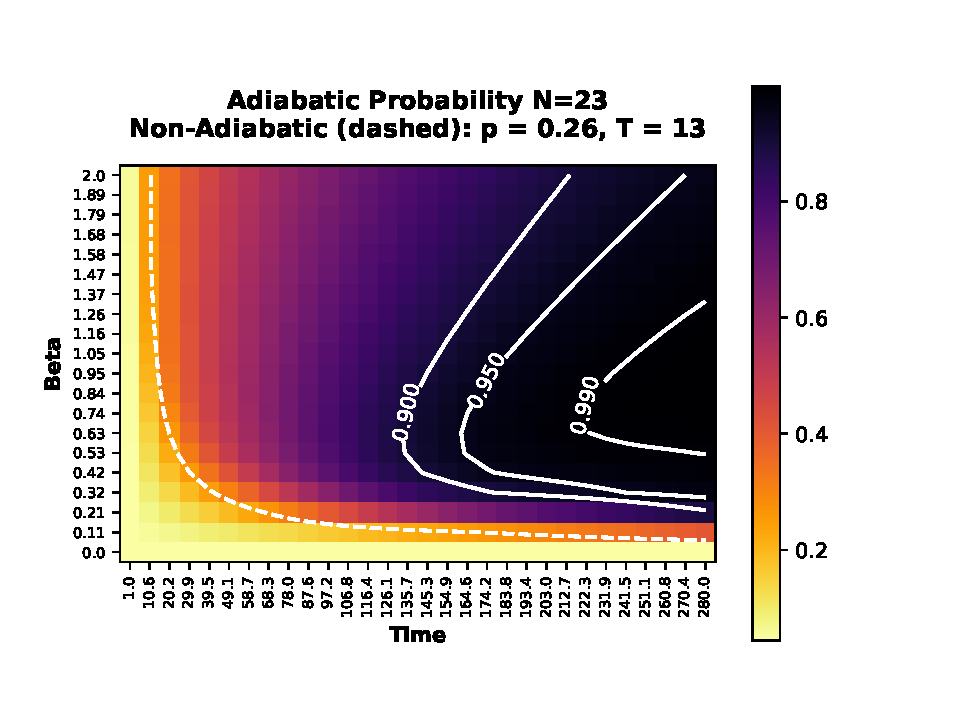
\includegraphics{./figures/23_probability_heatmap.pdf}%
\caption{Probability N=23 Time Dependent Approach}
\end{figure}

\subsection{Complete graph}


% % % % % % % %
% DISCUSSION
% % % % % % % %
\section{Discussion}
\subsection{So far}
\subsection{Future}


% % % % % % % % % % % % % % %
% APPENDIX: METHODS
% % % % % % % % % % % % % % %
\section{Methods}
In this section an overview of the computational methods is presented, focusing the attention on specific matters: \textit{Optimization Algorithm} used for determining the optimal $\gamma$-configuration for maximum probability, \textit{Schroedinger Solver} for the time dependent hamiltonian evolution and some additional parameters for the optimal \textit{Runge-Kutta Normalization Error}. Lastly computational reasoning for the \textit{2D - Probability Heatmap} are presented. \\

Most all numerical simulations were performed using \textbf{Python} being easy and flexible to sudden changes. Numerical methods such as optimization and ODE Solver come directly from python's native \textbf{Scipy}. In addition, a CPU-multiprocessing library, \textbf{Ray}, has been used to speed up the grid probability evaluation quite noticeably. 2D - Heatmap plots were created using python matplotlib, while additional plots were created with gnuplot.

\subsection{Optimization Algorithm}
In Section II a series of benchmark were performed to compare the standard Quantum-Walk algorithm to the Adiabatic-Quantum-Walk implementation (later simply named \textit{dynamic}). In order to determine which optimization algorithm fitted the best for the task, a number of possible algorithm were tested, such as \textit{shgo, dualannealing, minimize, LHSBH} and \textit{Basin-Hopping}. \\

Due to the oscillating nature of the probability (cfr figure) the scipy native \textbf{Basinhopping algorithm} was used. As the name suggests the algorithm performs a series of randomized hops, i.e. jumps, of the coordinates in order to find the true maximum (actually, the true \textit{minimum}). This fits particularly well with the series of maxima and minima of the probability function (for fixed $\gamma$) in the static algorithm (std QWAlgorithm). Snippets of the parameters used follow.

\begin{lstlisting}[xleftmargin=0cm]
	from scipy.optimize import basinhopping
	optimization = optimize.basinhopping()
	print(optimization)
\end{lstlisting}

\subsection{Schroedinger Solver}
In Section III we presented an evolution which is governed by a time-dependent hamiltonian, used to find the evolved state $|\psi(t)\rangle$. This is accomplished by solving the usual Schroedinger equation using Scipy's \textbf{integrate.solve\_ivp}, that provides a wide varieties of integrations methods. \\

As it's routine we used Runge-Kutta RK45, which as stated in the documentation it's a explicit Runge Kutta method of order 4(5). The error is controlled assuming fourth order accuracy, but steps are taken using the fifth-order accurate formula. In addition, the integrator is adaptive, meaning that the time step is chosen for optimal error control. Regarding the error, the algorithm provides two distinct parameters to set a targeted limit, namely the \textbf{relative (rtol)} and \textbf{absolute tolerances (atol)}. The first provides a relative accuracy, i.e. the number of digits, while the latter is used to keep the local error estimate below the threshold \textit{atol + rtol*abs(y)}. Determining the correct combinations of the two parameters is key for achieving the desired error. A few of those are presented in the following table, where a worst case scenario is used and the error is evaluated on the expected normalized state. \\

\begin{center}
\begin{adjustbox}{width=6cm}
\begin{tabular}{>{\rowmac}c>{\rowmac}c>{\rowmac}c>{\rowmac}c>{\rowmac}c<{\clearrow}} \toprule
    {rtol} & {atol} & {norm} &{error} & {comp time (s)}\\ \midrule
    e-3  & e-5 & 1.0851 & -0.0851 & 83.8\\
    \setrow{\bfseries} e-3  & e-6 & 1.0198 & -0.0198 & 19.5\\
    e-3  & e-7 & 1.0188 & -0.0188 & 19.4\\
    e-3  & e-8 & 1.0187 & -0.0187 & 19.5\\ \midrule

    e-4  & e-5 & 0.9988 & 1.16e-3 & 90.6\\
    e-4  & e-6 & 0.9996 & 3.98e-4 & 21.7\\
    e-4  & e-7 & 0.9996 & 4.13e-4 & 21.4 \\
    e-4  & e-8 & 0.9996 & 4.04e-4 & 21.5 \\ \midrule

    e-5  & e-5 & 0.9989 & 1.09e-3 & 82.8\\
    e-5  & e-6 & 0.9998 & 1.81e-4 & 20.5\\
    e-5  & e-7 & 0.9999 & 1.33e-4 & 20.6\\
    e-5  & e-8 & 0.9999 & 1.21e-4 & 20.8\\ \midrule

    e-6  & e-5 & 0.9998 & 2.48e-4 & 92  \\
    e-6  & e-6 & 0.9999 & 5.78e-5 & 22.6\\
    e-6  & e-7 & 0.9999 & 2.47e-5 & 23.2\\
    e-6  & e-8 & 0.9999 & 1.68e-5 & 23.2\\ \bottomrule

\end{tabular}
\end{adjustbox}
\end{center}



\subsection{2D - probability heatmap}


% If in two-column mode, this environment will change to single-column
% format so that long equations can be displayed. Use
% sparingly.
%\begin{widetext}
% put long equation here
%\end{widetext}

% figures should be put into the text as floats.
% Use the graphics or graphicx packages (distributed with LaTeX2e)
% and the \includegraphics macro defined in those packages.
% See the LaTeX Graphics Companion by Michel Goosens, Sebastian Rahtz,
% and Frank Mittelbach for instance.
%
% Here is an example of the general form of a figure:
% Fill in the caption in the braces of the \caption{} command. Put the label
% that you will use with \ref{} command in the braces of the \label{} command.
% Use the figure* environment if the figure should span across the
% entire page. There is no need to do explicit centering.

% \begin{figure}
% \includegraphics{}%
% \caption{\label{}}
% \end{figure}

% Surround figure environment with turnpage environment for landscape
% figure
% \begin{turnpage}
% \begin{figure}
% \includegraphics{}%
% \caption{\label{}}
% \end{figure}
% \end{turnpage}

% tables should appear as floats within the text
%
% Here is an example of the general form of a table:
% Fill in the caption in the braces of the \caption{} command. Put the label
% that you will use with \ref{} command in the braces of the \label{} command.
% Insert the column specifiers (l, r, c, d, etc.) in the empty braces of the
% \begin{tabular}{} command.
% The ruledtabular enviroment adds doubled rules to table and sets a
% reasonable default table settings.
% Use the table* environment to get a full-width table in two-column
% Add \usepackage{longtable} and the longtable (or longtable*}
% environment for nicely formatted long tables. Or use the the [H]
% placement option to break a long table (with less control than
% in longtable).
% \begin{table}%[H] add [H] placement to break table across pages
% \caption{\label{}}
% \begin{ruledtabular}
% \begin{tabular}{}
% Lines of table here ending with \\
% \end{tabular}
% \end{ruledtabular}
% \end{table}

% Surround table environment with turnpage environment for landscape
% table
% \begin{turnpage}
% \begin{table}
% \caption{\label{}}
% \begin{ruledtabular}
% \begin{tabular}{}
% \end{tabular}
% \end{ruledtabular}
% \end{table}
% \end{turnpage}

% Specify following sections are appendices. Use \appendix* if there
% only one appendix.
%\appendix
%\section{}

% If you have acknowledgments, this puts in the proper section head.
%\begin{acknowledgments}
% put your acknowledgments here.
%\end{acknowledgments}

% Create the reference section using BibTeX:
%\bibliography{basename of .bib file}

\end{document}
%
% ****** End of file apstemplate.tex ******
